\begin{remark}
    Section made from lectures done by Mike Kosch. Other sources are \citet{1995Itsp} --- chapter 9 \& parts of chapter 13.
\end{remark}

\section{Solar wind}
The hot solar corona (plus solar flares and coronal mass ejections) overcomes gravity and results in a wind, i.e.\ hot plasma (95\% protons and electrons) radiating outwards from the Sun to fill the interplanetary vacuum. We gain information about the magnetic field by looking at the polarization of light.

\subsection{Collisionless plasma?}
We take a look back at \cref{eq:magnitude_magnetic_field} to make sure we remember it. Due to the frozen in condition, the magnetic field strength of the sun at L1 is much higher than the geometry would suggest. The mean free path, i.e.\ the average distance between collisions is
\begin{equation*}
    \ell=\frac{k_{B}T}{\sqrt{2}\pi d^2p}
\end{equation*}
where \(p\) is pressure and \(d\) is the distance between protons.\\
\begin{minipage}[t]{.5\linewidth}
    \textbf{Is the solar wind collisionless?}\\
    Proton: \(d=\num{1.65e-15}\) m\\
    Pressure: \(p=\num{1e-4}-\num{1e-15}\) Pa\\
    Fast solar wind: \(T_i\approx 1500\) K, \(\ell >\num{1.7e13}\) m\\
    Slow solar wind: \(T_i\approx \num{8e5}\) K, \(\ell >\num{9e15}\) m
\end{minipage}
\begin{minipage}[t]{.5\linewidth}
    \textbf{Is the ionosphere (\SI{250}{\kilo\metre}) collisionless?}\\
    Proton: \(d=\num{1.65e-15}\) m\\
    Pressure: \(p=\sim\num{1e-4}\) Pa\\
    Oxygen amount \(=16\) \\
    \(T_i\approx 1500\) K, \(\ell >\num{1.1e12}\) m\\
    \(1 AU \approx\num{1.5e11}\) m
\end{minipage}

\subsection{Frozen in magnetic flux}
When investigating the frozen in magnetic flux, we will need Ohm's law, \(\gf{j}=\sigma\left(\gf{E}+\gf{u}\times\gf{B}\right)\), the condition of collisionless plasma giving \(\sigma=\infty \) and therefore \(\gf{E}=-\gf{u}\times\gf{B}\), i.e.\ convection applies.
\begin{equation*}
    \gf{j}=\sigma\left(\gf{E}+\gf{u}\times\gf{B}\right)
\end{equation*}
and then the Lorentz' force give
\begin{equation*}
    \gf{F}=q\left(\gf{E}+\gf{u}\times\gf{B}\right)=q\gf{E}+\gf{I}\times\gf{B}
\end{equation*}
\begin{equation*}
    \frac{\gf{j}}{\sigma|_\infty}=0=\gf{E}+\gf{u}\times\gf{B}
\end{equation*}
From this we get that if we have no electric field we also have no velocities, or if we do have velocities, we will also have an electric field. How is this possible? The answer is blowing in the wind, or rather, magnetic field lines is stuck in the solar wind.

\subsection{What controls the solar wind?}
Typical solar wind forces at 1 AU are a plasma pressure of \(p=nk_{B}T\) (\(\sim \num{1.3e-13}\)), a magnetic pressure of \(p=B^2/2\mu_0\) (\(\sim \num{1.4e-11}\)) and a dynamic pressure of \(p=\rho u^2\) (\(\sim \num{1.7e-9}\)). We see that at this point, the dynamic pressure is by far the dominating process.

\section{SuperDARN radars}
Coherent scatter radars with Tx peak power \(=\SI{9.6}{\kilo\watt}\) at \(8\)--\(\SI{20}{\mega\hertz}\). The range is \(\sim 1000\)--\(\SI{3000}{\kilo\metre}\) with a range resolution of \(15\)--\(\SI{45}{\kilo\metre}\). The time resolution is \(\sim\SI{120}{\second}\) and you have 16 beams. 12 radars is located in the southern hemisphere, while in the northern hemisphere there are 22 radars.

Their main objective is to observe plasma flow in the ionosphere at \(200\)--\(\SI{300}{\kilo\metre}\) altitude. The radars can only see backscatter with right angles to the field lines. Field aligned plasma irregularities like stritiations and scintillations have frequencies of
\begin{equation*}
    \Delta f=\frac{\Delta v}{c}f_0
\end{equation*}

Coherent backscatter is what the technique is called, or alternatively Bragg scattering. Bragg's law for crystals (coherent scatter) is given as
\begin{equation}\label{eq:L8_bragg_scatter}
    n\lambda=2d\sin\theta
\end{equation}
From the SuperDARN radars, we get data to add to the convection flow maps.

\section{Thin current sheets}
Discontinuities of magnetic electric field result in currents. From Ampere's law we have
\begin{equation*}
    \oint_C\gf{B}\cdot\tn{d}\gf{\ell}=\mu_0\iint_S\gf{j}\cdot\tn{d}\gf{S}=\mu_0I_{enc}
\end{equation*}
Regions of distinctly different magnetic field are separated by current sheets, e.g.\ the magnetopause of magnetotail neutral sheet. Ampere's law applies, hence the current sheets. Current sheets are ``thin'', e.g.\ \SI{100}{\kilo\metre} (versus \(10\)--\(100 R_E\)).

\subsection{Magnetopause/magnetotail position}
The location of the magnetopause is where the solar wind dynamic pressure balances the magnetosphere magnetic pressure.
We find the distance to the ring current and assume \(B_z<0\) to get the balancing equation
\begin{equation*}
    nmu^2=\frac{{(2\cdot 13)}^2}{2\mu_0}=\frac{4{\left(\frac{B_0}{r^3}\right)}^2}{2\mu_0}
\end{equation*}
where \(B_0=\num{31000}\si{\nano\tesla}\), \(\mu_0=4\pi 10^{-7}\), \(u\) is the solar wind speed, \(n\) the solar wind density and \(m=m_p\). We end up with an expression for the distance \(r\) given as
\begin{equation*}
    r=\sqrt[6]{\frac{2B_0^2}{nmu^2\mu_0}}=9.85 R_E
\end{equation*}

Looking at the magnetopause in closer detail, we first make the assumption that \(\gf{B}=\gf{0}\). When the particles meet the magnetic field of the Earth, they start gyrating, ions down and electrons up. This gives a current moving down, and we look at the magnitude by checking how many, first ions, that crosses any given horizontal line (flux) (\cref{fig:L8_magnetopause_flux}). We know that flux is given as
\begin{equation*}
    \xi=2rnu
\end{equation*}
and for current we have
\begin{equation*}
    I=2r nuq=\xi q
\end{equation*}
For a loop going through our region of interest we get
\begin{equation*}
    \mu_0 I=B_z+0+0+0 \Rightarrow I=\frac{B_z}{\mu_0}
\end{equation*}
\begin{equation*}
    \frac{B_z}{\mu_0}=2r nuq\Rightarrow r=\frac{mu}{qB_z}
\end{equation*}
\begin{equation*}
    \underset{\substack{\uparrow \\ \tn{magnetic}\\ \tn{pressure}}}{\frac{B_z^2}{2\mu_0}}=\underset{\substack{\uparrow \\ \tn{dynamic}\\ \tn{pressure}}}{mu^2}
\end{equation*}
We may also take a look at how thick the magnetopause is.
\begin{equation*}
    r=\frac{mu}{qB},\quad B=\frac{B_0}{r^3}\approx \SI{31}{\nano\tesla}
\end{equation*}
\begin{equation*}
    \Rightarrow r=\SI{16.8}{\kilo\metre}
\end{equation*}
where we have used \(u=\SI{500}{\kilo\metre/\second}\), \(m=m_p\) and \(q\) is the elementary charge.
\begin{figure}[t]
    \centering
    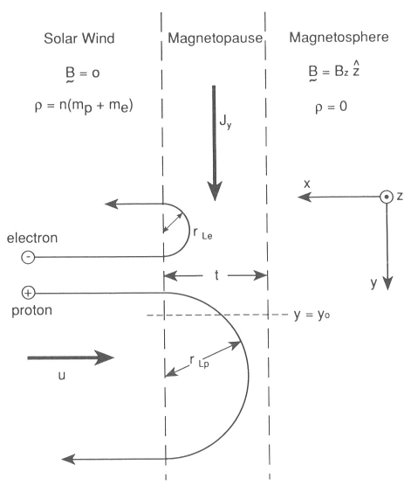
\includegraphics[width=.4\linewidth]{bilder/L8_magnetopause_flux.jpeg}
    \caption{Flux of ions and electrons crossing through a line in the \(xy\)-plane in the magnetopause.}\label{fig:L8_magnetopause_flux}
\end{figure}

\section{The geomagnetic tail}
Here we find reservoirs of plasma and energy, and this is associated with substorms. The magnetic field strength in the near/far Earth tail lobe is generally \(B=20/\SI{10}{\nano\tesla}\) respectively.

\subsection{Plasma beta (\(\beta \))}
Plasma beta is defined as
\begin{align*}
    \tn{plasma beta}&=\frac{\tn{plasma thermal pressure}}{\tn{magnetic pressure}}\\
    \beta&=\frac{nk_{B}T}{B^2/2\mu_0}
\end{align*}
We can find the width of the magnetotail by looking at the total magnetic flux close to the Earth (polar cap) and compare this to the total magnetic flux in the tail. This yields
\begin{align*}
    \phi=\int \gf{B}\cdot\tn{d}\gf{S},\quad \phi_{pc}=\phi_T\\
    \Rightarrow \phi=BA
\end{align*}
For the polar cap, this can fairly easily be found
\begin{equation*}
    \phi_{pc}=2B_0\left[\pi{\left(R_E\sin\theta_{pc}\right)}^2\right]
\end{equation*}
where \(\theta_{pc}\sim \SI{15}{\degree}\) and the term \(2B_0\) appears because of the dipole approximation, \(B_0\) at the equator and \(2B_0\) at the pole. With a value of \(B_T=\SI{20}{\nano\tesla}\) or \(B_T=\SI{10}{\nano\tesla}\) this gives us (found from \(B_T^2/2\mu_0=nk_B(T_e-T_i)\))
\begin{equation*}
    r_T=20 R_E\quad\tn{and}\quad r_T=29 R_E
\end{equation*}

\subsection{Tail flaring}
Tail flaring is an effect we see due to the interaction of solar wind vs.\ magnetic pressure. This give an unstable situation similar to what you would see from a flag blowing in strong wind.

The total mass of the magnetosphere can be found to be, using the numbers that gave us \(r_T=29R_E\) and a length of \(1000R_E\) and a number density \(n=\num{0.3e6}\) we have
\begin{equation*}
    \tn{mass}=1000R_E\pi{\left(29R_E\right)}^2nm_p\approx \num{3.42e5}\si{\kilo\gram}=342\tn{ tons}
\end{equation*}
Here, we have used \(nmu^2\sin\theta=B^2/2\mu_0\) due to the widening of the magnetotail.

\section{Magnetic reconnection \& the Dungey cycle}
\subsection{\(B_z\) negative}
For the solar wind, the Reynolds number get very high. The conductivity is practically infinite, scale lengths are large and velocities are huge. The Reynolds number is defined as
\begin{equation*}
    Re=\frac{VL}{\eta},\quad\eta=\frac{1}{\mu_0\sigma_0}
\end{equation*}
For magnetic reconnection we need the frozen-in conditions to break down, i.e.~\(Re\leq 1\), which give diffusion. We look at the induction equation
\begin{equation*}
    \p{t}{\gf{B}}=\nabla\times\left(\gf{u}\times\gf{B}\right)+\frac{\nabla^2\gf{B}}{\mu_0\sigma_0}
\end{equation*}
We assume \(u\approx 0\), hence
\begin{equation*}
    \p{t}{\gf{B}}=\frac{\nabla^2\gf{B}}{\mu_0\sigma_0}
\end{equation*}
Let \(\gf{B}||\mathbf{x}\) so that \(\p{y}{B_x}=0=\p{x}{B_x}\).
\begin{equation*}
    \p{t}{B_x}=\frac{1}{\mu_0\sigma_0}\p{zz}{B_x}=0
\end{equation*}
We get the diffusion equation and we see that the \(x\)-component of \(B\) is constant along the \(z\)-direction. The steady state assumption gives us
\begin{equation*}
    \p{t}{B_x}=0\Rightarrow\p{z}{B_x}=\tn{constant}
\end{equation*}
We now impose an electrical field, included in Ohm's law from the frozen-in condition
\begin{equation*}
    E_y=-u_{z}B_x
\end{equation*}
Faraday's law tells us that
\begin{equation*}
    \nabla\times\gf{E}=\p{t}{\gf{B}}=0
\end{equation*}
From this we see that since \(B_x\) is constant through time then \(E_y\) is constant. Therefore \(u_z\) must be constant. In the diffusive zone we have \(E_y=j_y/\sigma_0\), and here we make use of Ampere's law to look at the current
\begin{align*}
    \oint\gf{B}\cdot\tn{d}\gf{\ell}&=\mu_0 I\\
    B_{x}x+0+\left(-B_x\right)\left(x\right)+0&=\mu_0 I\\
    2B_{x}x&=\mu_0 I
\end{align*}
\begin{equation*}
    \therefore j_y=\frac{I}{x2\ell}=\frac{B_x}{\ell\mu_0}
\end{equation*}
Now, notice that the electric field should be constant in our region, both in the diffusive zone and the convective zone. Combining the expressions for the two cases where \(E_y\) appears gives us
\begin{equation*}
    E_y=\frac{B_x}{\ell\mu_0\sigma_0}=-u_{z}B_x
\end{equation*}
\begin{equation}\label{eq:L8_ell_relation_reynold}
    u_z\mu_0\sigma_0\ell=1
\end{equation}
which is the Reynolds number. What this means is that the frozen-in condition does not apply in this scenario, and we allow for plasma to move across magnetic filed lines.

But where does the energy go? It will be transferred to the electrons, and we get a hint by looking at Fick's law of diffusion
\begin{equation*}
    J=-\mu_0k_{B}T\p{x}{n}
\end{equation*}
where \(J\) is the flux and \(n\) is the number density. The size of the electrical field that the solar wind carries can be found from looking at the velocity of the solar wind and the strength of the magnetic field:
\begin{equation*}
    E=-u_{sw}B_{sw}=\SI{400}{\kilo\metre/\second}\times\SI{6}{\nano\tesla}=\SI{2.4}{\milli\volt/\metre}
\end{equation*}
The polar cap potential can be found from this. We again use that the polar cap reaches \(\theta=\SI{15}{\degree}\) from the pole, giving a radius of \(r_{pc}=\theta R_E=\SI{1500}{\kilo\metre}\). Thus
\begin{equation*}
    \Phi_{pc}=E2r_{pc}=\SI{8}{\kilo\volt}
\end{equation*}

We can find the distance downstream at where the reconnection takes place. Again we use \(u_{sw}=\SI{400}{\kilo\metre/\second}\) and the time it takes the field lines to convect over the polar cap is simply \(t=2r_{pc}/v_{pc}=2\times\SI{1500}{\kilo\metre}/\SI{330}{\metre/\second}\approx 10^4\si{\second}\).
\begin{equation*}
    D_x=u_{sw}t\approx 600R_E
\end{equation*}
We might assume a polar cap potential of \(\Phi_{pc}=\SI{60}{\kilo\volt}\). If we use a width of the tail of \(D=50R_E\) with \(B_{sw}=\SI{5}{\nano\tesla}\) we end up with a potential across the tail of
\begin{equation*}
    \Phi=ED=B_{sw}u_{sw}D=\SI{640}{\kilo\volt}
\end{equation*}
What we notice is that this potential might be ten times the potential at the polar cap, meaning most particles do not get trapped and hence do not precipitate down to the Earth.
\begin{figure}[t]
    \centering
    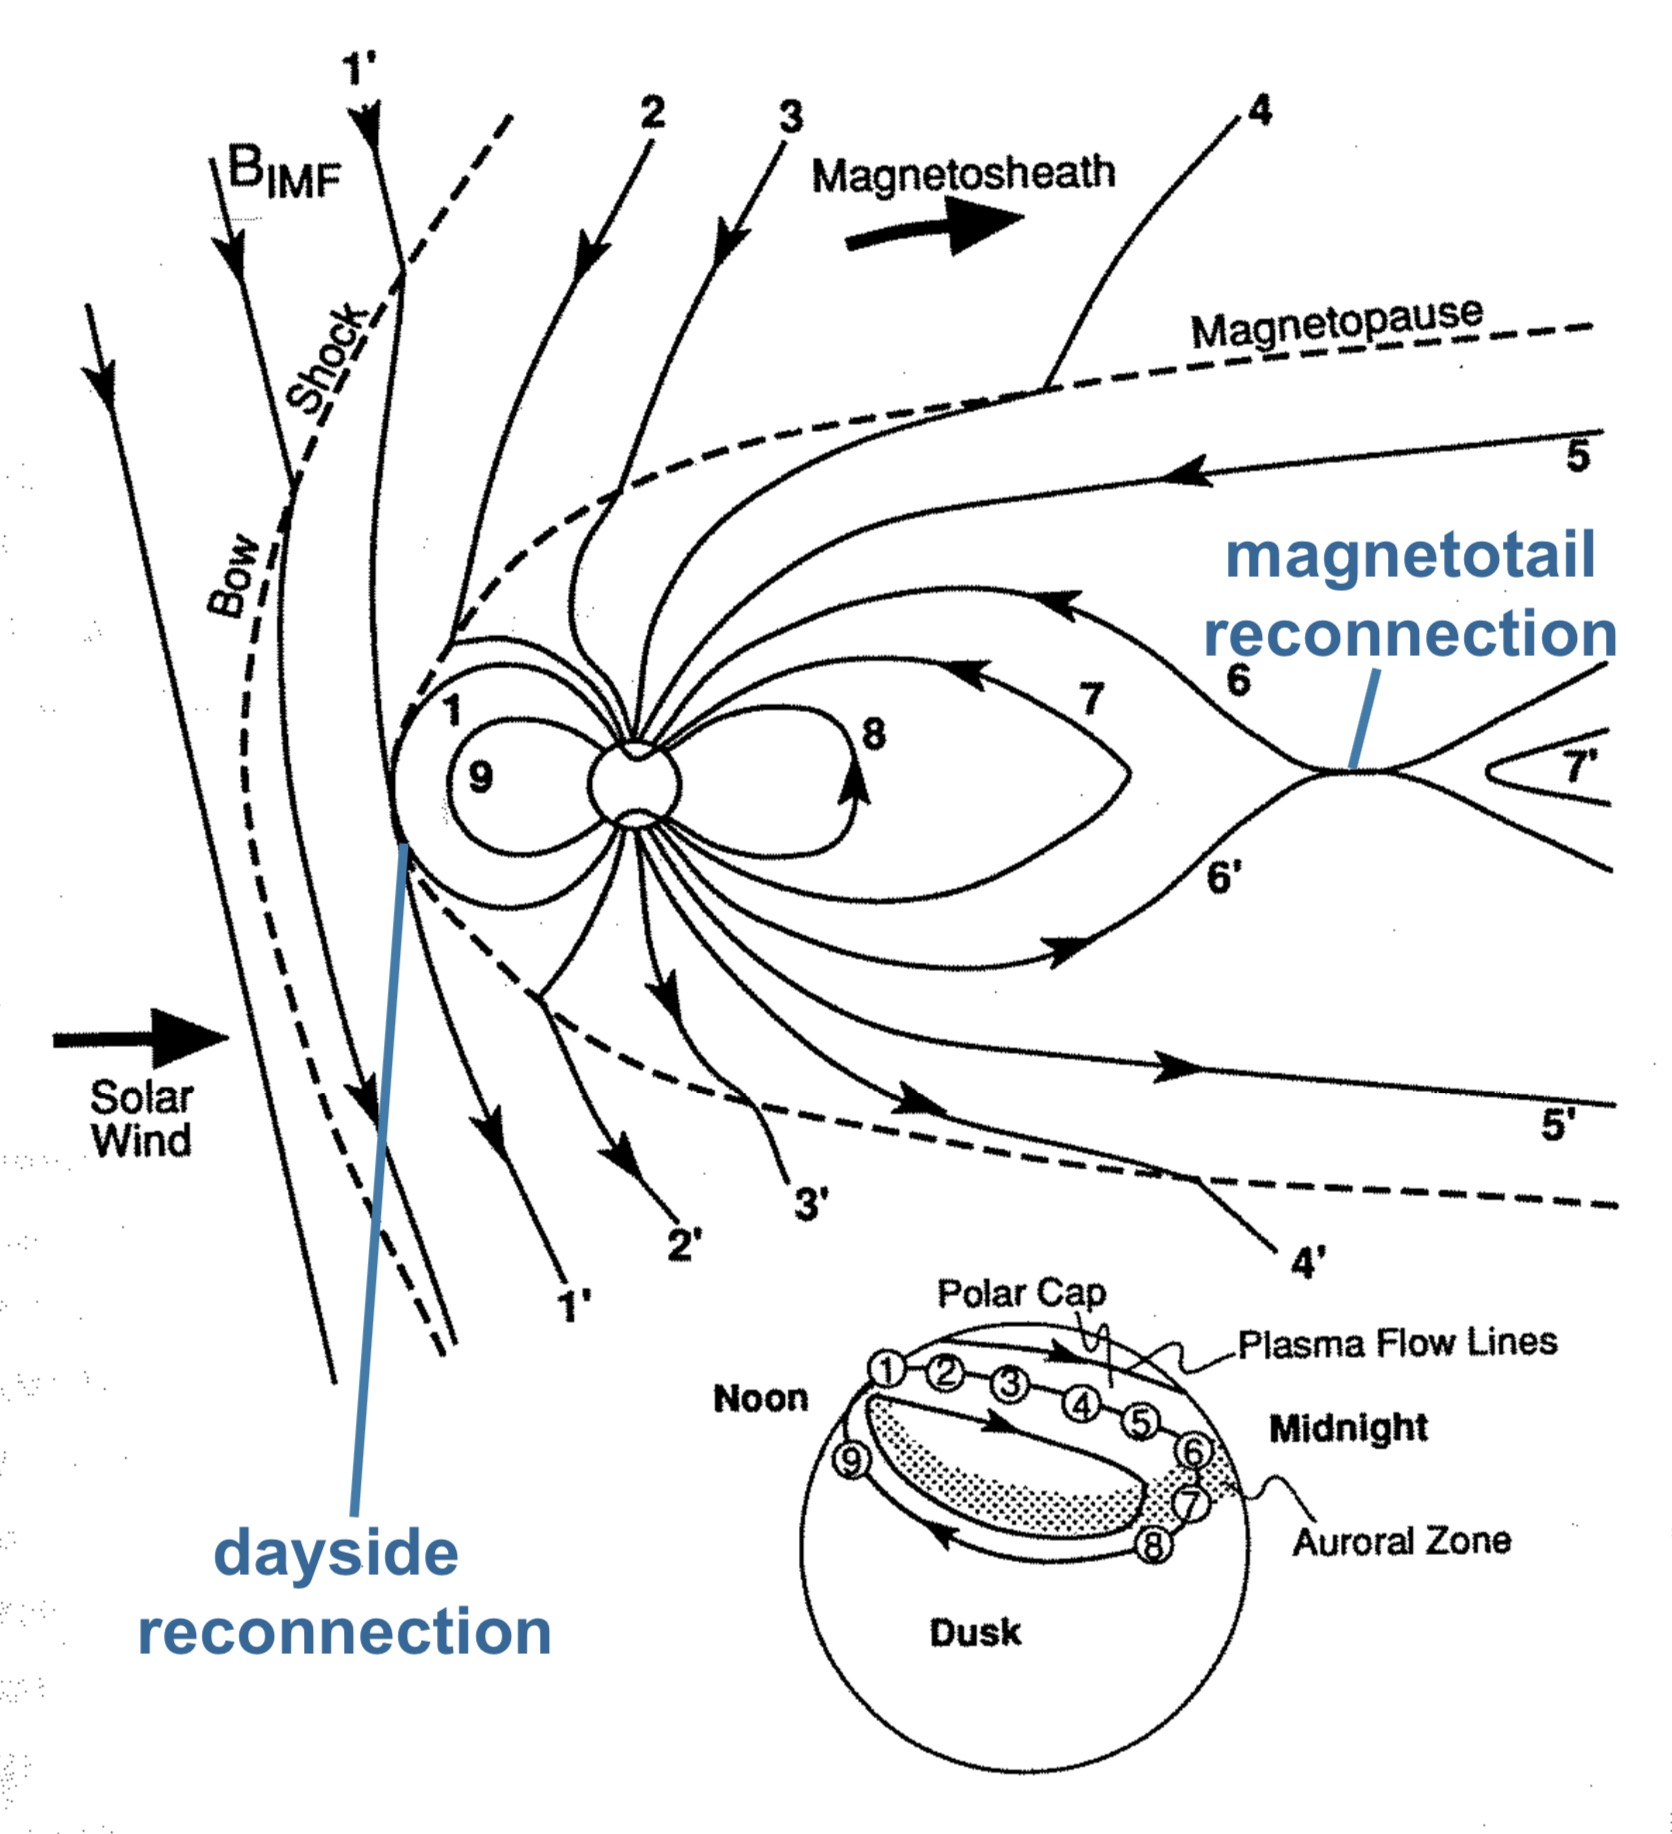
\includegraphics[width=.4\linewidth]{bilder/L8_dungey_cycle.jpg}
    \caption{The Dungey cycle.}\label{fig:L8_dungey_cycle}
\end{figure}

\subsection{Reconnection asymmetry}
For \(B_y<0\) or \(B_y>0\) we get different convection patterns. The reconnection asymmetry we get for \(B_y<0\) (points towards dusk) is a banana that lies on the dusk side, and vice versa. We also see a shift of the dayside OCB in the direction of the \(B_y\) component.
\begin{figure}[t]
    \centering
    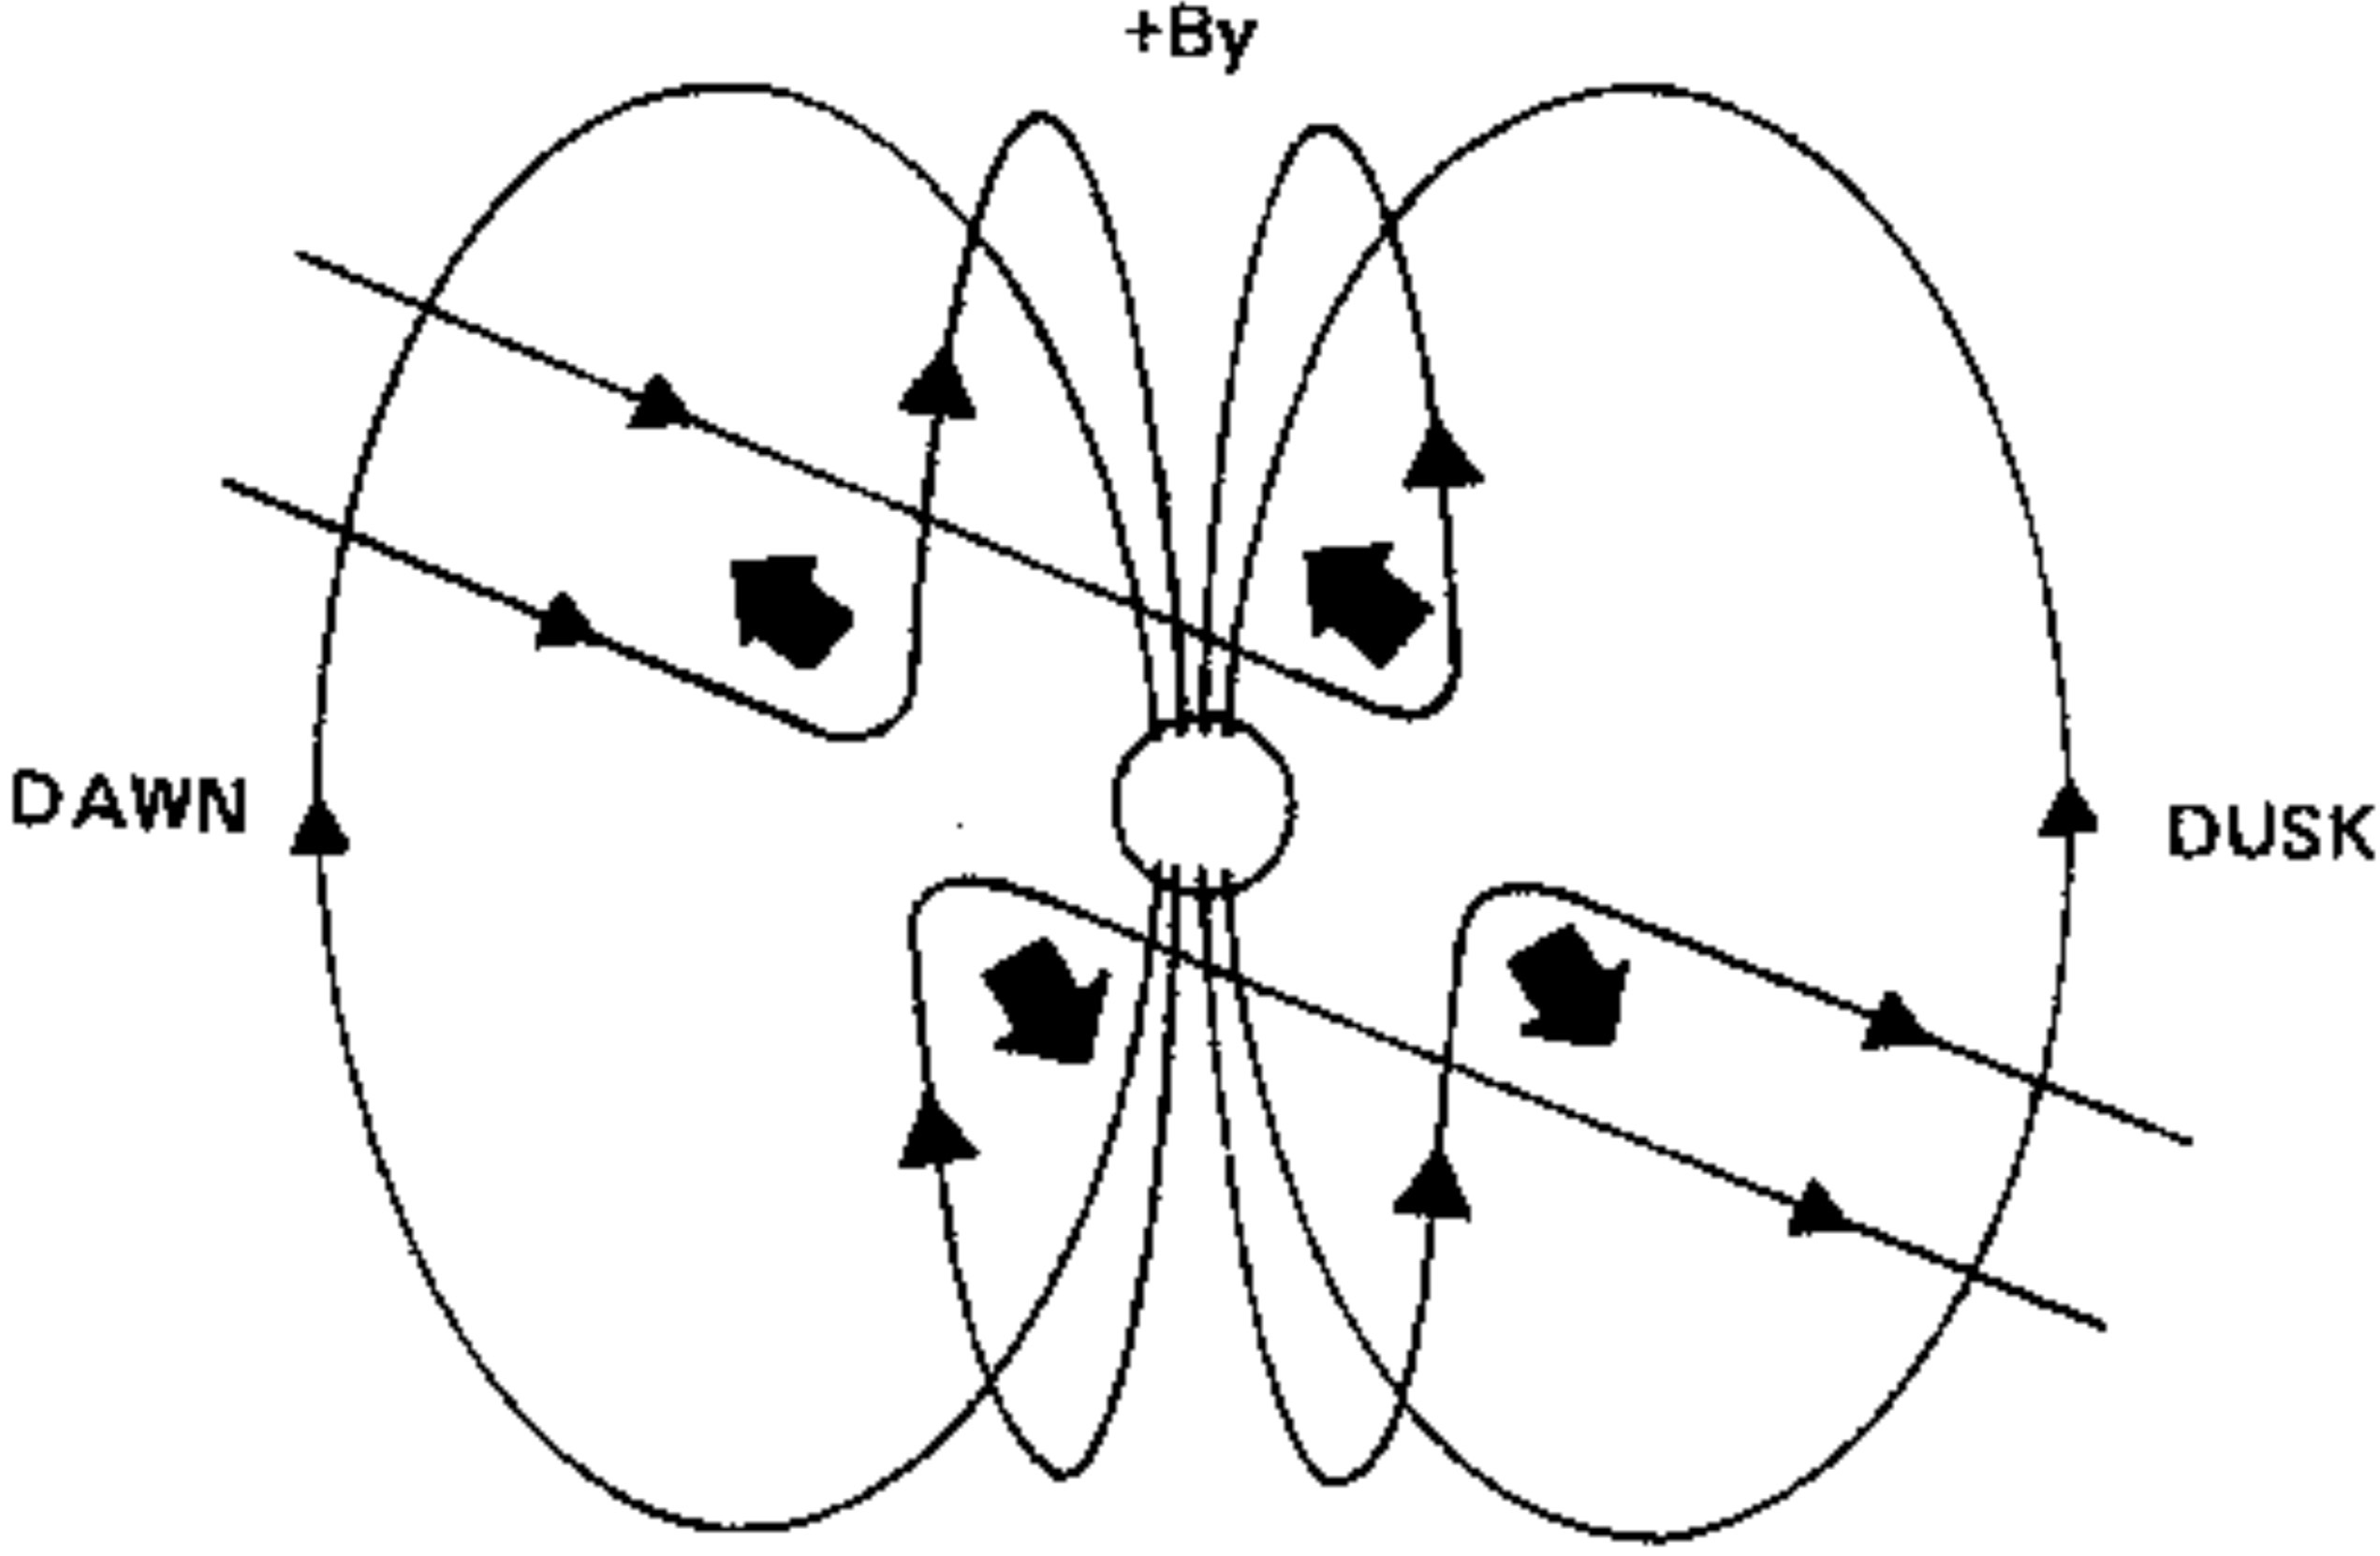
\includegraphics[width=.4\linewidth]{bilder/L8_by_asymmetry.jpg}
    \caption{\(B_y\) positive seen from the sun.}\label{fig:L8_by_asymmetry}
\end{figure}

\subsection{\(B_z\) positive}
For positive IMF we also get reconnection, but at a much lower efficiency. It reconnects with the magnetic field of the Earth at bit behind the poles where closed lines have downward components. As usual, we also see reconnection on the nightside where the magnetic lines from the Earth meets up.

\subsection{Fluid description of reconnection}
Here, we will develop the MHD fluid descriptions of magnetic reconnection. The model will be time-stationary and two-dimensional. We start with the Sweet-Parker solution shown in \cref{fig:L8_mag_recon}. This is a basic \(x\)-line configuration. The shaded diffusion region is \(2L\) long and \(2\ell \) wide, where \(L\gg\ell \). We assume for simplicity that the inflow and outflow parameters are symmetrical. A reasonable assumption in the tail, not so much for the magnetopause. The electric field is spatially uniform and points out of the page, so that
\begin{equation*}
    E=u_{i}B_i=u_{o}B_o
\end{equation*}
We also assume that the flow is incompressible, i.e.\ that \(\rho_i=\rho_o=\rho \), and from conservation of mass we get
\begin{equation}\label{eq:L8_ell_relation_L}
    u_{i}L=u_o\ell
\end{equation}
We now turn our attention to the energy. We look at how the kinetic energy gained by the outflowing plasma compare to the electromagnetic energy flowing into the diffusion regions. The electromagnetic-energy inflow rate per unit area is given by the Poynting flux
\begin{equation*}
    |\gf{S}|=|\gf{E}\times\gf{H}|=\frac{EB_i}{\mu_0},\quad\gf{H}=\frac{\gf{B}}{\mu_0}
\end{equation*}
\begin{equation*}
    |\gf{S}|=\frac{u_{i}B_i^2}{\mu_0}
\end{equation*}
The mechanical energy out is given by the gain in kinetic energy of the outflowing plasma. The rate of energy gain per unit area in the incident flow is
\begin{equation*}
    \Delta W=\frac{1}{2}\rho_f u_i\left(u_o^2-\cancelto{0}{u_i^2}~~~\right)
\end{equation*}
where \(\rho_f\) is the flow rate.
\begin{align*}
    \frac{u_{i}B_i^2}{\mu_0}&=\frac{1}{2}\rho u_{i}u_o^2\\
    u_o^2&=\frac{2B_i^2}{\mu_0\rho},\quad v_A=\frac{B}{\sqrt{\mu_0\rho}}\\
    u_o^2&=2v_A^2
\end{align*}
where \(\rho \) denotes mass density. We use the expression from \cref{eq:L8_ell_relation_L} in the above equation to obtain
\begin{equation*}
    \frac{u_i^2L^2}{\ell^2}=2v_A^2
\end{equation*}
\begin{equation*}
    u_i=\frac{\sqrt{2}v_A\ell}{L}
\end{equation*}
From \cref{eq:L8_ell_relation_reynold}, we have that the Reynolds number is given as \(Re=1=\mu_0\sigma\ell u_i\) in the diffusion region. We substitute for \(\ell \) and obtain
\begin{equation*}
    u_i^2=\frac{\sqrt{2}v_A}{\mu_0\sigma L}
\end{equation*}
or equivalently
\begin{equation*}
    u_i=v_A\sqrt{\frac{\sqrt{2}}{Re}}
\end{equation*}
where \(v_A\approx\SI{510}{\kilo\metre/\second}\) is the solar wind speed. What we end up with is that in all solar-system plasmas for which \(Re\) is very large, the incoming velocity is way too low compared to the velocity we know the solar wind to have. Using \(\nu=5/3, T_i=\num{12e5}\si{\kelvin},T_e=\num{1.4e5}\si{\kelvin}, m_i=m_p\) we get \(v_s=\SI{53}{\kilo\metre/\second}\).

This was solved by Petchek, with the geometry shown in \cref{fig:L8_reconnection_new_solution}, when he realized that most of the plasma does not need to flow through the diffusion region to get accelerated, but can be accelerated in the region where MHD is still valid, in the convection region. We must have shock waves to obtain the force required to get reconnection in the diffusion region, shock waves that are connected to the diffusion region and that remain fixed in space. This removes the bottleneck caused by requiring that all plasma should flow within a length \(\ell \) in the midplane. The diffusion region is still important in this solution since it is here the reconnection has to happen, but, the region can be vanishingly small. Its size will not even enter our calculations.
\begin{figure}[t]
    \centering
    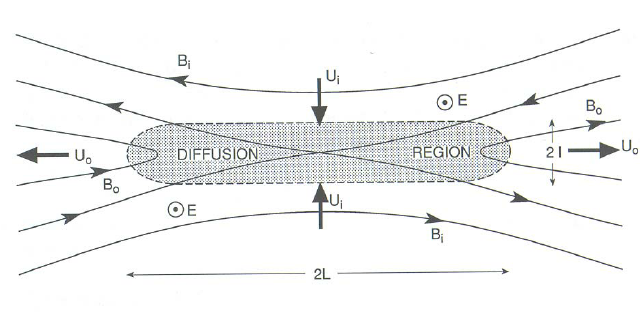
\includegraphics[width=.6\linewidth]{bilder/L8_mag_recon.png}
    \caption{The Sweet-Parker solution to magnetic reconnection.}\label{fig:L8_mag_recon}
\end{figure}
\begin{figure}[t]
    \centering
    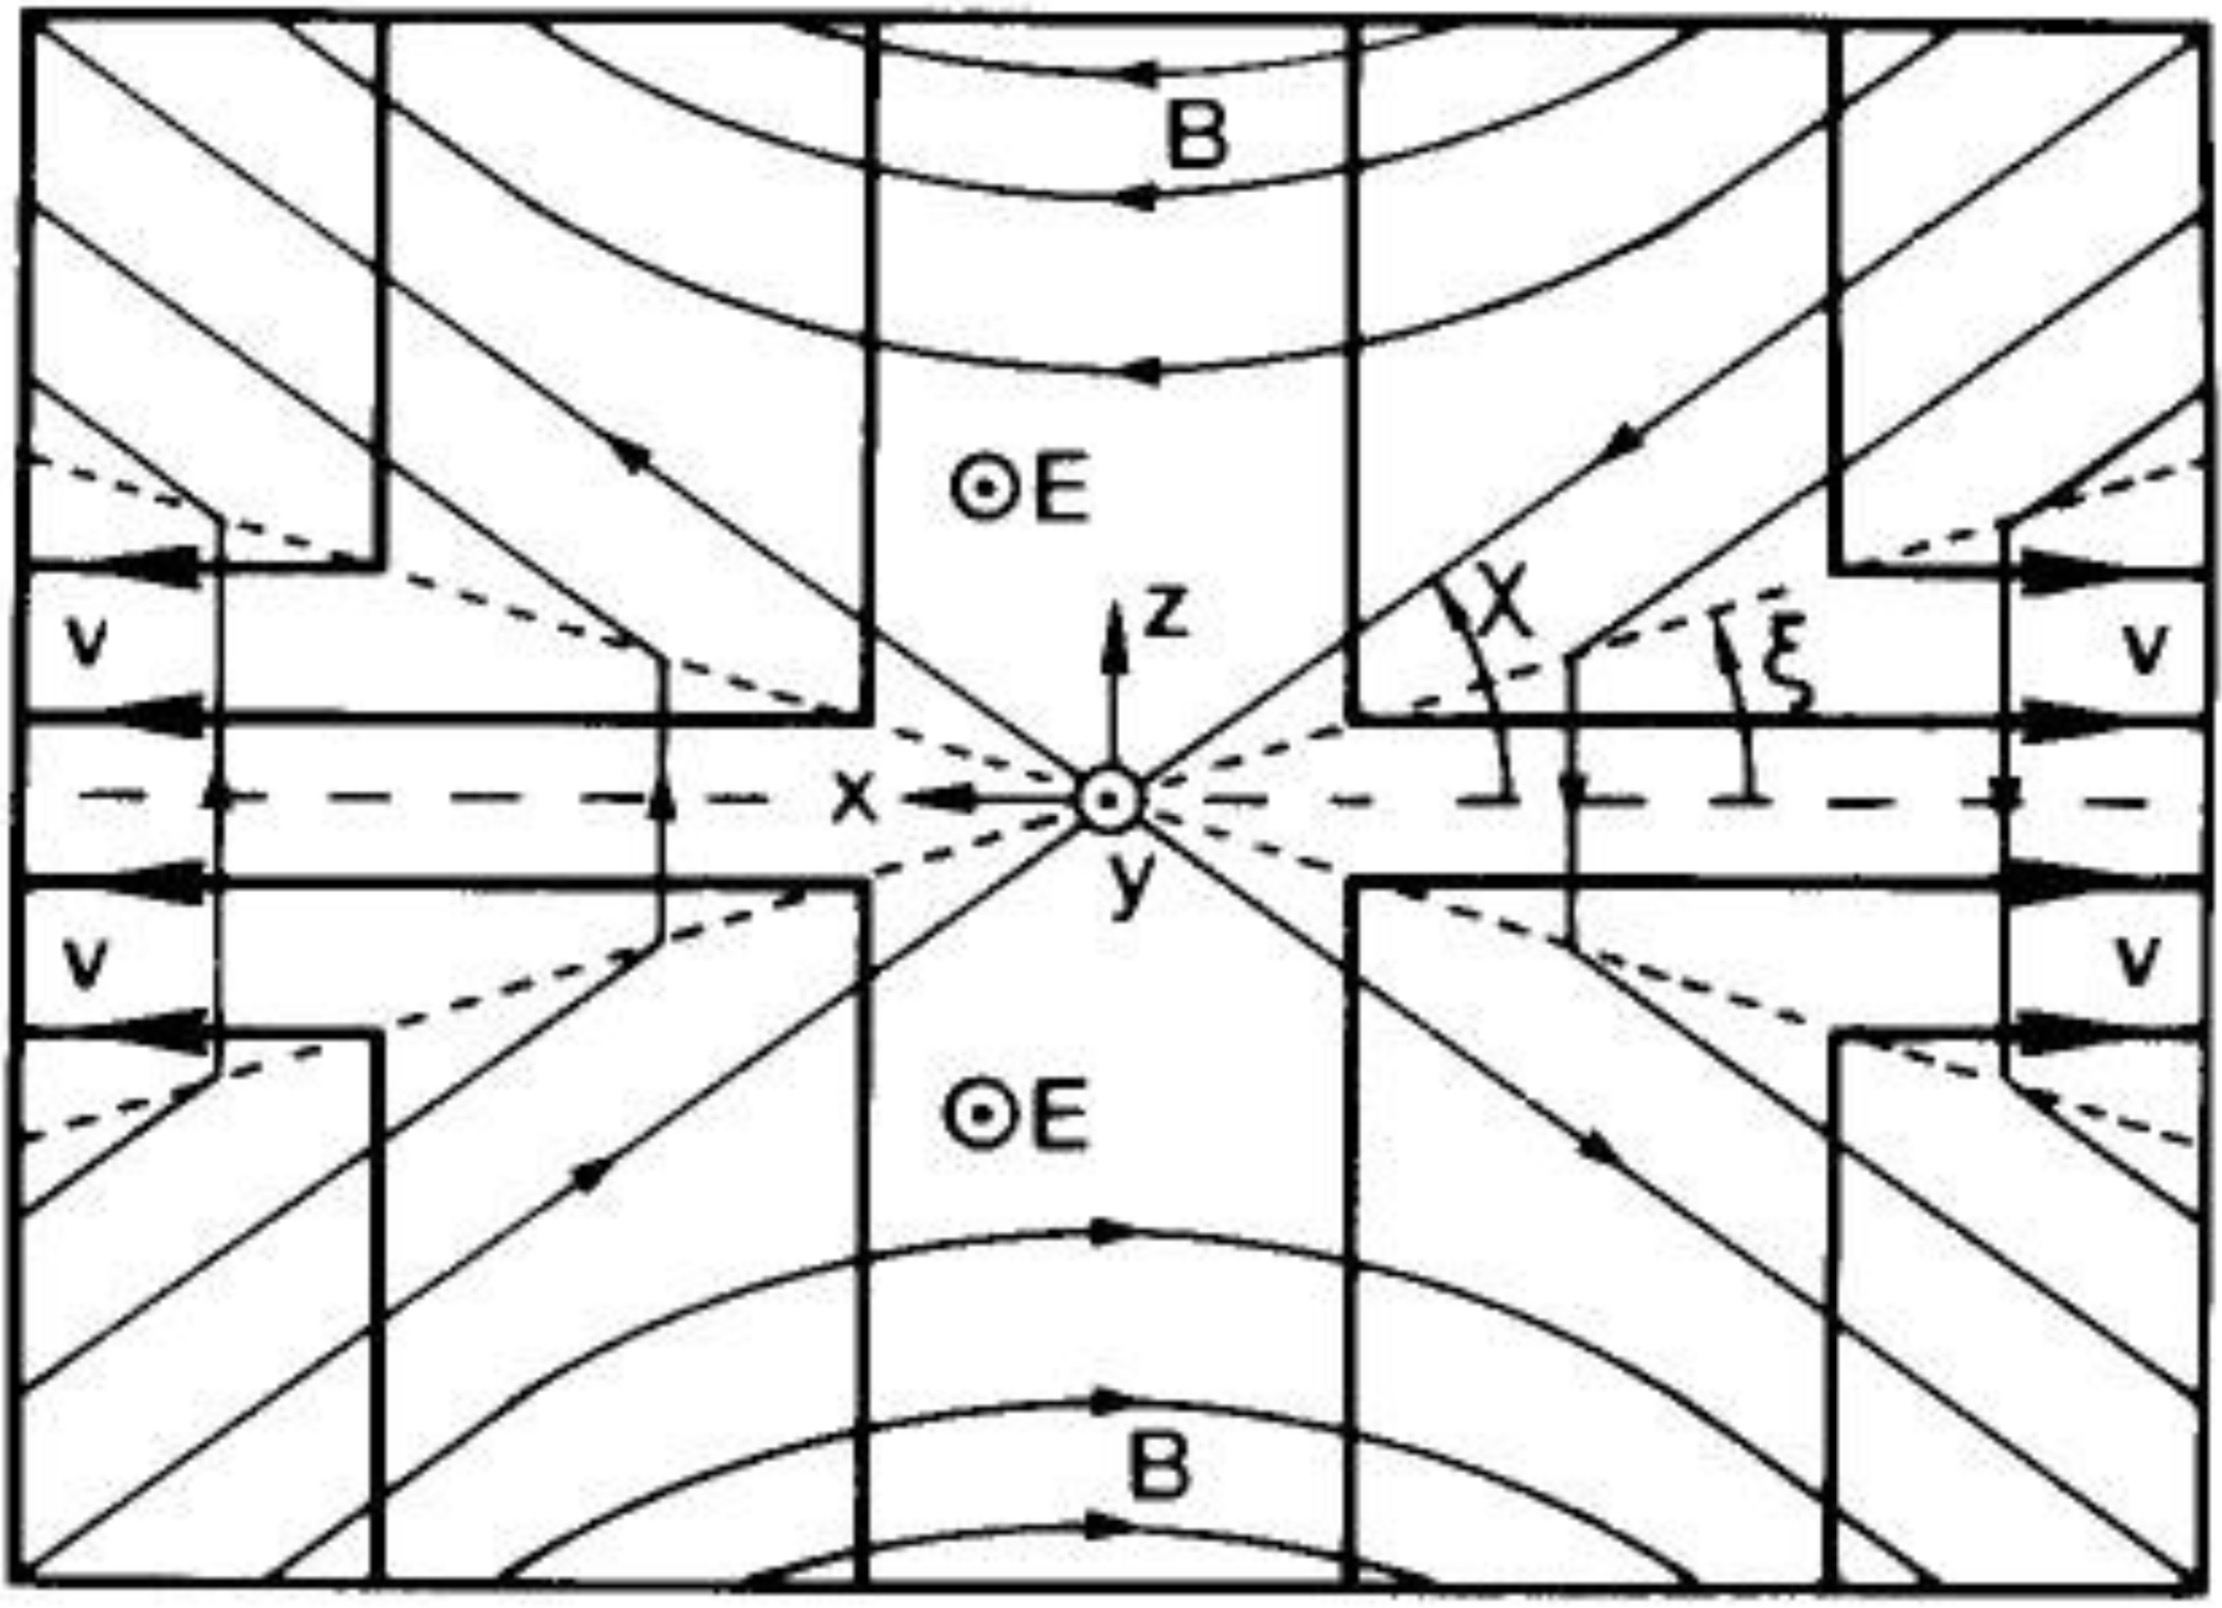
\includegraphics[width=.7\linewidth]{bilder/L8_reconnection_new_solution.jpg}
    \caption{The geometry of the new solution to reconnection proposed by Petchek.}\label{fig:L8_reconnection_new_solution}
\end{figure}

Shock waves form in gases and fluids in front of supersonic objects, or in front of objects within supersonic flows. Across the shock wave front, the properties of the gas (density, temperature, field strength, flow speed) change suddenly. If the kinetic energy is reduced, the thermal energy will be increased (\(k_{B}T\)). Generally, shocks are not adiabatic, i.e.\ not reversible. This implies energy dissipation, i.e.\ that entropy is increasing.

But how do shocks form in collision less plasma? Collisions are not required to form shocks. Electrostatic and electromagnetic forces can act. A shock must conserve mass, energy and momentum as well as obey the MHD equations.

Let \(Q\) be density and \(\gf{F}\) the flux. For conservation of mass, energy and momentum we get
\begin{equation*}
    \p{t}{Q}+\nabla\cdot\gf{F}=0
\end{equation*}
By assuming steady state and 1-dimension only we have
\begin{equation*}
    \p{x}{F_x}=0,\qquad\left(\gf{F}_{u}-\gf{F}_{d}\right)\cdot\f{x}=0,\qquad\left[F_x\right]=0
\end{equation*}
We then impose the MHD criteria of continuity
\begin{equation*}
    \p{x}{\rho u_x}=0,\qquad\left[\rho u_x\right]=0
\end{equation*}
From Maxwell's equations we have \(\nabla\cdot\gf{B}=0\), and by also enforcing that tangential \(\gf{E}_T\) must be preserved, i.e.~\(\nabla\times\gf{E}=-\p{t}{\gf{B}}\) we assume the steady state and frozen in condition \(\gf{E}=-\gf{u}\times\gf{B}\).

A termination shock is where gas of fluid goes from supersonic to subsonic without an intervening object, and it is similar to water in a sink. This may happen because the plasma is cooling
\begin{equation*}
    v_s=\sqrt{\frac{k_B\left(\gamma T_i+T_e\right)}{m_i}}
\end{equation*}
A termination shock forms where the solar wind meets the interstellar medium (\(T=10\)--\(\num{10000}\) K) at a distance of \(\sim 75\)--\(90\) AU\@.

\subsection{Bow shock}
\begin{enumerate}[\(\bullet \)]
    \item thickness: 100--1000\si{\kilo\metre}
    \item distance: \(13.5R_E\)
    \item solar wind mean free path \(>\) 1 AU
\end{enumerate}

\section{Open closed field lines}
\subsection[Viscous coupling]{Viscous coupling (K\&R p. 264)}
Another factor that let particles through to our magnetosphere is viscous coupling, although this is far less important compared to magnetic reconnection. It is a term used to include any process other than magnetic reconnection that can transport momentum across the magnetopause. It can include kinetic processes --- such as anomalous particle diffusion  via wave-particle interactions --- and large-scale fluid interactions. In the latter case, particles in the solar wind that drifts on the flanks of the magnetosphere can be caught by frictional forces due to a Kelvin-Helmholtz instability, or magnetopause distortions resulting from traveling pressure variations in the magnetosheath. A third concept --- impulsive plasma penetrations --- has also been proposed to contribute to this viscosity. These processes contribute to approximately 10--20\% of the particles that enter.

Flux transfer events are when we get an increase in particles that is moved into our magnetosphere.

\subsection[Ion upflow]{Ion upflow (K\&R p. 277)}
Imagine a magnetosheath consisting of \(\tn{H}^+\) that entered the magnetosphere and has just mirrored at low altitude on the field line labeled 2 in \cref{fig:L8_dungey_cycle}. The ion moves up the field line, and as it encounters weaker magnetic fields, its parallel velocity increases. Soon the pitch angle is close to zero, and if it is moving quickly it will soon reach the magnetopause again and reenter the magnetosheath. This may happen by the time the field line has convected to the position of of the field line labeled 3. A more slowly moving ion will exit the magnetosphere father down the tail, where lines 4 and 5 crosses the magnetopause. If the ion is sufficiently slow, it will still be on the magnetospheric portion of the filed line when the line reaches position 6, and what happens next depends on weather the ion is tailward or earthward of the \(x\)-line when the field line reconnects. If it is earthward, the ion will enter the current sheet on a closed field line and follow a Spieser-type orbit before it is accelerated towards the Earth.

We can quantitatively derive a relation among the speed at which the particle moves, the cross-tail potential drop, and the distance to the \(x\)-line to find what energy particles will enter the plasma sheet earthward of the neutral line. Let the distance to the ``pinch off''/\(x\)-line be \(L_x\) and assume the magnetic field lines to be straight. The time it takes an ion to reach the critical point will then be given as
\begin{equation*}
    t=\frac{L_x}{v_{||}}
\end{equation*}
We have the size of the electric field given as
\begin{equation*}
    E=\frac{\Phi}{2R_T}
\end{equation*}
and by combining this by use of the \(\gf{E}\times\gf{B}\) drift we get
\begin{equation*}
    t=\frac{2R_T^2B_T}{\Phi}
\end{equation*}
and
\begin{equation*}
    v_{||}=\frac{\Phi L_x}{2R_T^2B_T}
\end{equation*}
\begin{equation*}
    \therefore W_c=\frac{m}{2}{\left(\frac{\Phi L_x}{2R_T^2B_T}\right)}^2
\end{equation*}
where \(B_T\) is the lobe field strength and \(W_c\) is the critical particle energy. We may use \(L_x=100R_E, \Phi=\SI{53}{\kilo\volt},R_T=26R_E,B_T=\SI{10}{\nano\tesla}\).
\begin{equation*}
    \Rightarrow v_{||}=\SI{21}{\electronvolt}
\end{equation*}
Since we have \(T_i=T_e\approx\SI{1500}{\kelvin}=\SI{0.15}{\electronvolt}\) in the upper atmosphere, we see that there is a second order of magnitude less than what they need to gain to escape.

\subsection{Radiation belts}
The inner belt goes from \(0.01\)--\(1.5R_E\) with \(E_P\sim <\SI{100}{\mega\electronvolt}\) (protons) while the outer belt goes from \(3\)--\(10R_E\) with \(E_P\sim <\SI{10}{\mega\electronvolt}\) (electrons). The outer radiation belt is highly variable, but since the inner belt is on permanently closed magnetic field lines it is much more stable.

The particles accumulate because the loss is particularly weak here. Inner belt is caused by cosmic rays. They ionize what ever they come in contact with. The outer belt is mostly caused by reconnection, making it more unstable. In just a matter of hours, the outer radiation belt may die out and load up again.

\section{Auroral oval}
We expect to see symmetrical structures in the northern and southern hemispheres, but due to difficulties in knowing which filed lines maps to where between the hemispheres and the \(B_y\) skewing, among other things, this has been difficult to see.

Hall conductance gives the size of the magnetic field, but not the energy dissipation. The Birkeland currents are parallel to the magnetic field.

Region 1 currents (\cref{fig:L8_all_currents}) are more poleward than region 2 currents. Both can either be up or down, the region only tells you about latitude. The Harang\footnote{\href{https://nbl.snl.no/Leiv_Harang}{Leiv Harang}} discontinuity is where region 1 and 2 do not match up. Generally, auroras correspond to upward currents since this is where the downward electron flow is.

Hall current (electrojets) exists because it is a transition between collisionless and collisional plasmas.
\begin{figure}[t]
    \centering
    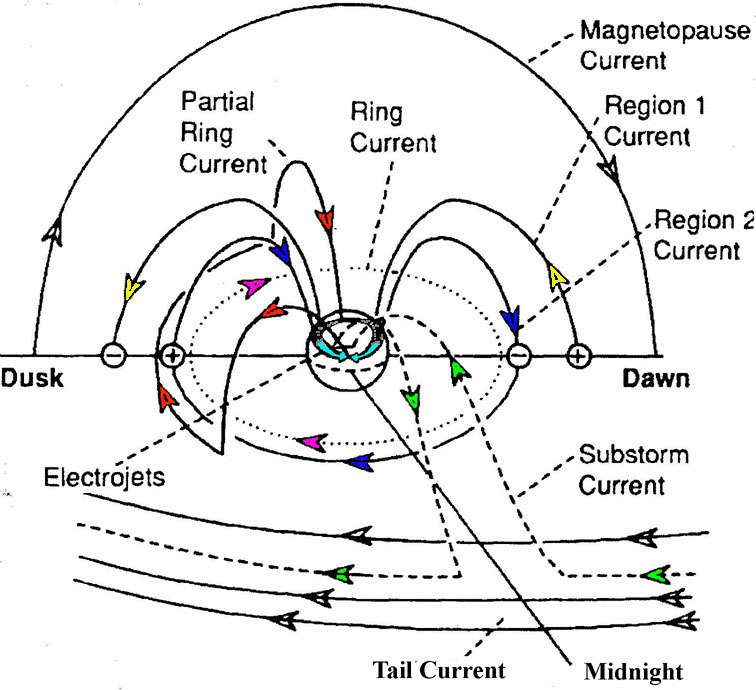
\includegraphics[width=.4\linewidth]{bilder/L8_all_currents.jpg}
    \caption{The currents we find in the magnetosphere. Depending on the precipitation and ionization the current may go straight past the Earth or down to the Earth and up.}\label{fig:L8_all_currents}
\end{figure}

\section{Substorms}
\subsection{Near Earth neutral line (NENL)}
The best developed model of substorms is the near-earth neutral-line (NENL) model. This model attempts to provide an internally consistent explanation for most magnetospheric phenomena, but does not attempt to explain many ionospheric observations. In the NENL model, a substorm begins when a southward turning of the IMF activates dayside reconnection. The start of the substorms come from particles precipitating from the NENL, illustrated in \cref{fig:L8_NENL_plasmoids}. The \(X\)-line is assumed to be inactive. Dayside magnetic flux from the Earth connects to the IMF and is transported over the polar caps by the solar wind, where it is added to the outer portions of the tail lobes. The removal of this flux from the dayside initiates a convective flow of plasma toward the reconnection region, but the flow is retarded by the finite conductivity of the ionosphere at the foot of the field lines. Because of this, the magnetospheric return flow is unable to balance the rate at which flux reconnects, and the dayside magnetopause erodes earthward.

Dayside erosion increases magnetopause flaring, thus increasing the dynamic pressure on the boundary, and this pressure reduces the flaring angle, compressing the tail until a corresponding increase in tail-lobe magnetic pressure balances the external pressure.

\subsection{Plasmoids (O-line)}
The unique feature of the NENL model is the formation of a \emph{plasmoid} that is ejected from the plasma sheet during the expansion and recovery phase of a substorm. The formation of a plasmoid is a direct consequence of the substorm growth phase that initiate the substorm. When the magnetic field lines bulge out again, these structures arise in the magnetotail behind the NENL\@.
\begin{figure}[t]
    \centering
    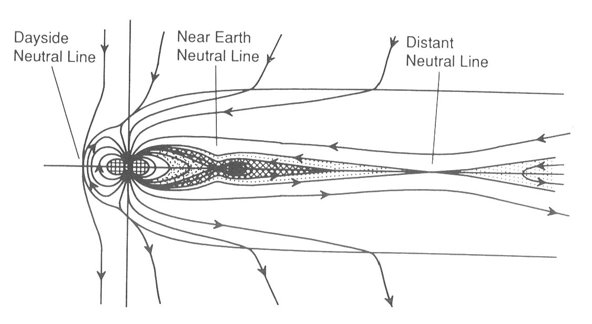
\includegraphics[width=.7\linewidth]{bilder/L8_NENL_plasmoids.jpeg}
    \caption{The location of the near Earth neutral line in the magnetotail and a plasmoid right behind it.}\label{fig:L8_NENL_plasmoids}
\end{figure}

\section{Important equations}
A summary of the most equations from this section is
\coloredeqq{
    \begin{aligned}
        p&=nk_{B}T&&\tn{---~~~Plasma pressure}\\
        p&=\frac{B^2}{2\mu_0}&&\tn{---~~~Magnetic pressure}\\
        p&=\rho{}u^2=nmu^2&&\tn{---~~~Dynamic pressure}\\
        \oint\gf{B}\cdot\tn{d}\gf{\ell}&=\mu_0I&&\tn{---~~~Ampere's law}\\
        \gf{F}&=q\left(\gf{E}+\gf{u}\times\gf{B}\right)&&\tn{---~~~Lorentz' law}\\
        \gf{j}&=\sigma\left(\gf{E}+\gf{u}\times\gf{B}\right)&&\tn{---~~~Ohm's law}\\
        \tn{Rm}&=\mu_0\sigma{}UL&&\tn{---~~~Magnetic Reynolds number}
    \end{aligned}
}